\section{Results and Tests}

\subsection{Energy mode}
The first part of the assignemnt focused on implementing and testing the routines described in the methodology. Following are tests cases explained in the form of inputs and expected/actual outputs. It is assumed that the LEDs, button, and GPIO-clock have already been set up properly, as described in section (INSERT SECTION HERE).
Screenshots from the eAProfiler energy monitor have been included for illustration.

	\subsubsection{Polling}
	\emph{Input: } branch link only to polling \\
	\emph{Expected output: } high energy use, in the upper scale of the energy monitor \\
	\emph{Actual output: } as expected, with an average current of 3.74 mA
	
	\begin{center}
		\begin{figure}[H]
			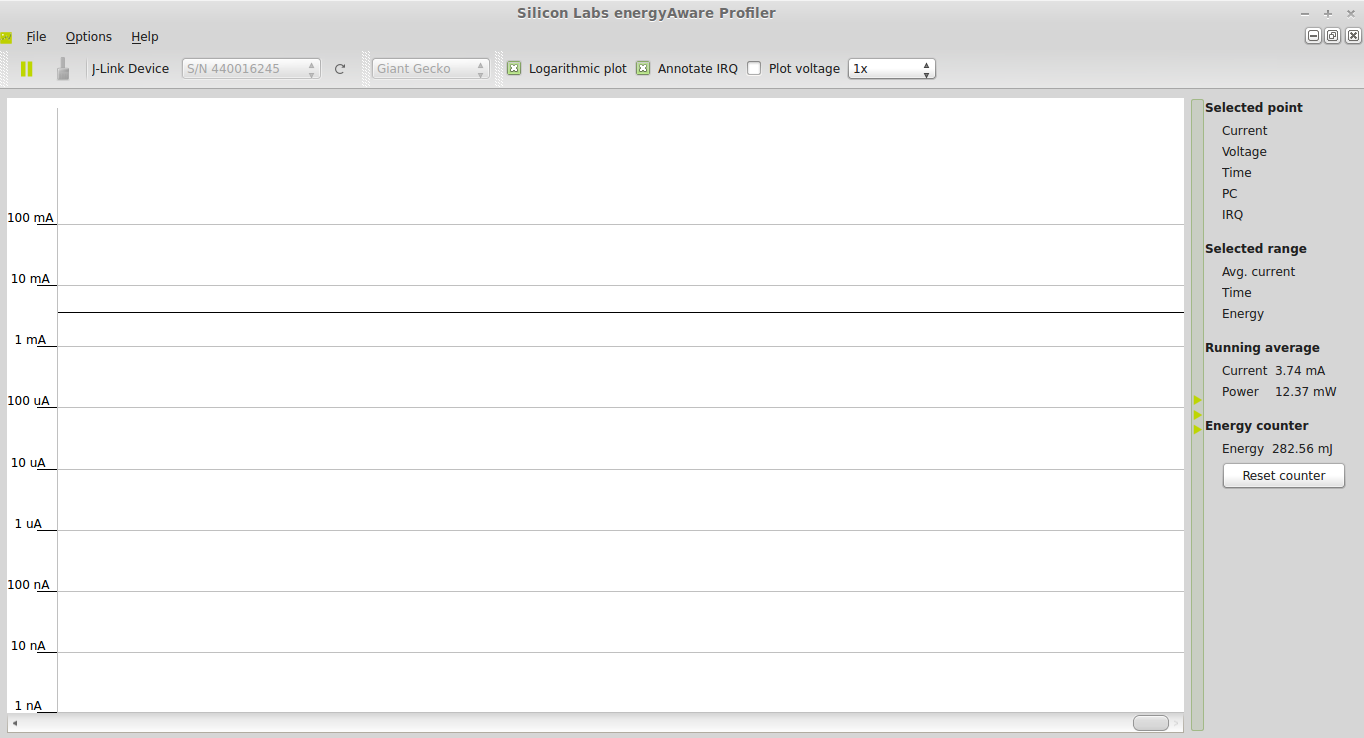
\includegraphics[width=\textwidth]{fig/polling.png}
			\caption{Polling}
		\end{figure}
	\end{center}
	
	
	\subsubsection{Interrupt without energy mode}
	\emph{input: } 
	branch link only to $setup_interrupts$ function, then execute WFI condition code \\
	\emph{expected output: }
	lower energy use than polling, but still relatively high \\
	\emph{actual output: }
	Average current hovering around 1.22 mA
	
	\begin{center}
		\begin{figure}[H]
		
			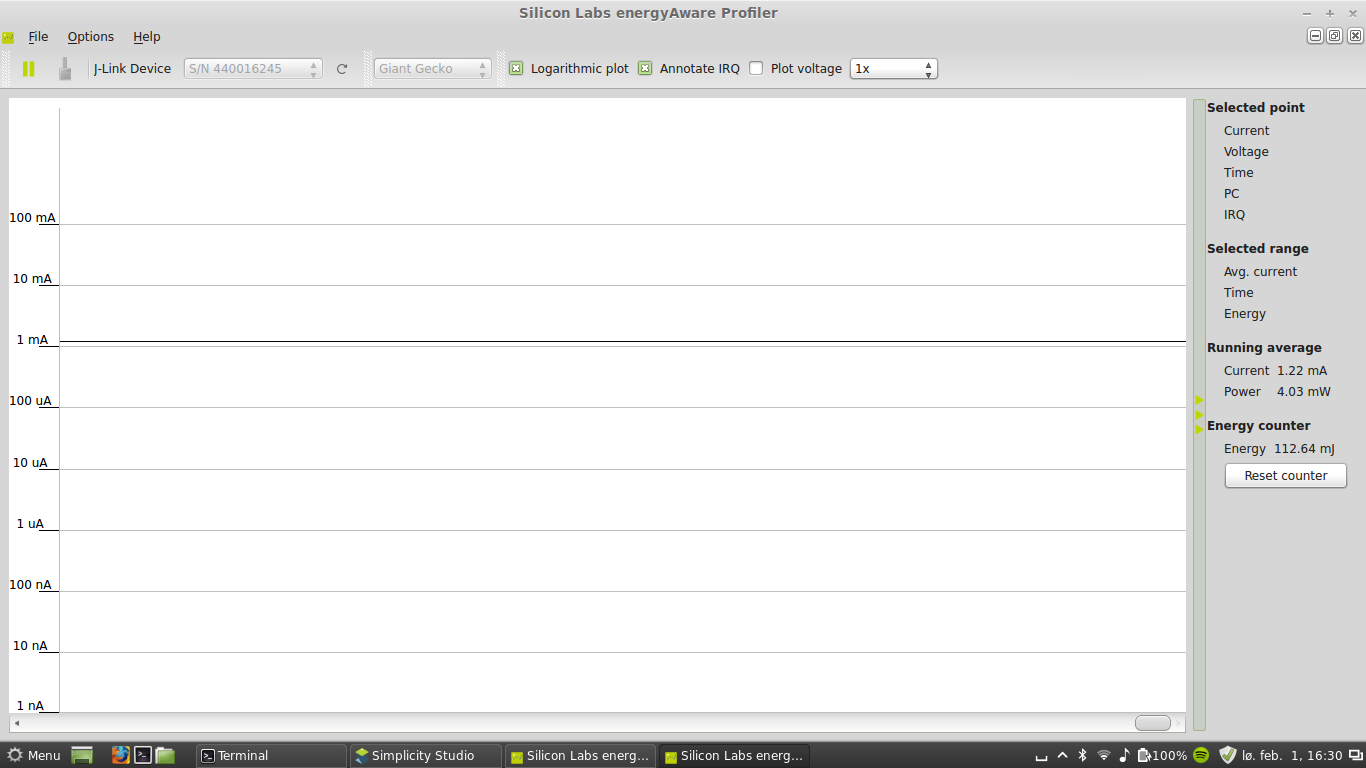
\includegraphics[width=\textwidth]{fig/InterruptOnly.png}
			\caption{Interrupt without energy mode}
		\end{figure}
	\end{center}

		
	\subsubsection{Interrupt with energy mode}
	\emph{input: }	branch link to $setup_interrupts$ and $setup_energy_mode$, then execute WFI condition code \\
	\emph{expected output: } dratically lowered energy consumption \\
	\emph{actual output: } As expected, with average current of 1.94$\mu$s \\
	
	\begin{center}
		\begin{figure}[H]
			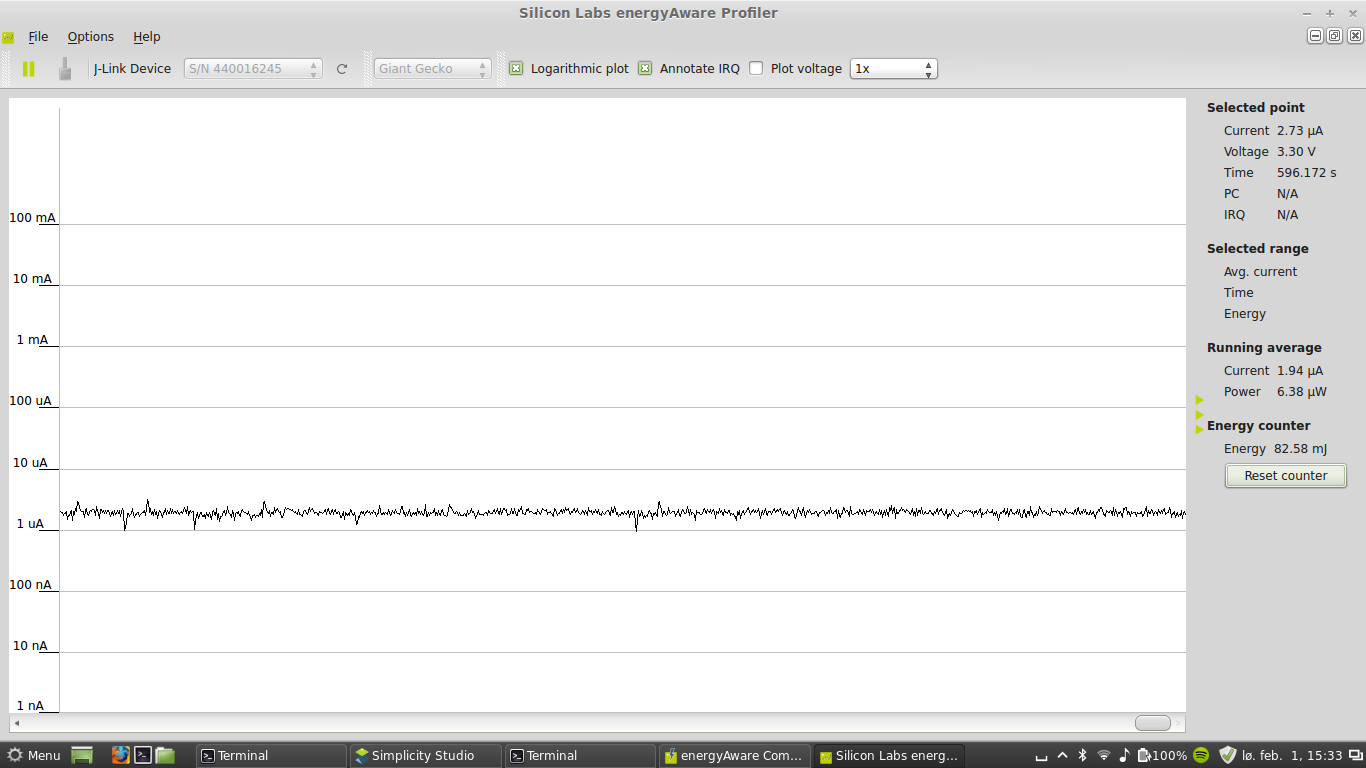
\includegraphics[width=\textwidth]{fig/interruptsAndEnergy.png}	
			\caption{Interrupt with energy mode}
		\end{figure}
	\end{center}
	
	\subsubsection{Interrupt and energy mode with button pressed}
	\emph{Input: } Same setup as above, but with the test of briefly pressing a button \\
	\emph{Expected output: } Brief spike in energy usage, and return to normal when button is released \\
	\emph{Actual output: } As expected
	
	\begin{center}
		\begin{figure}[H]
			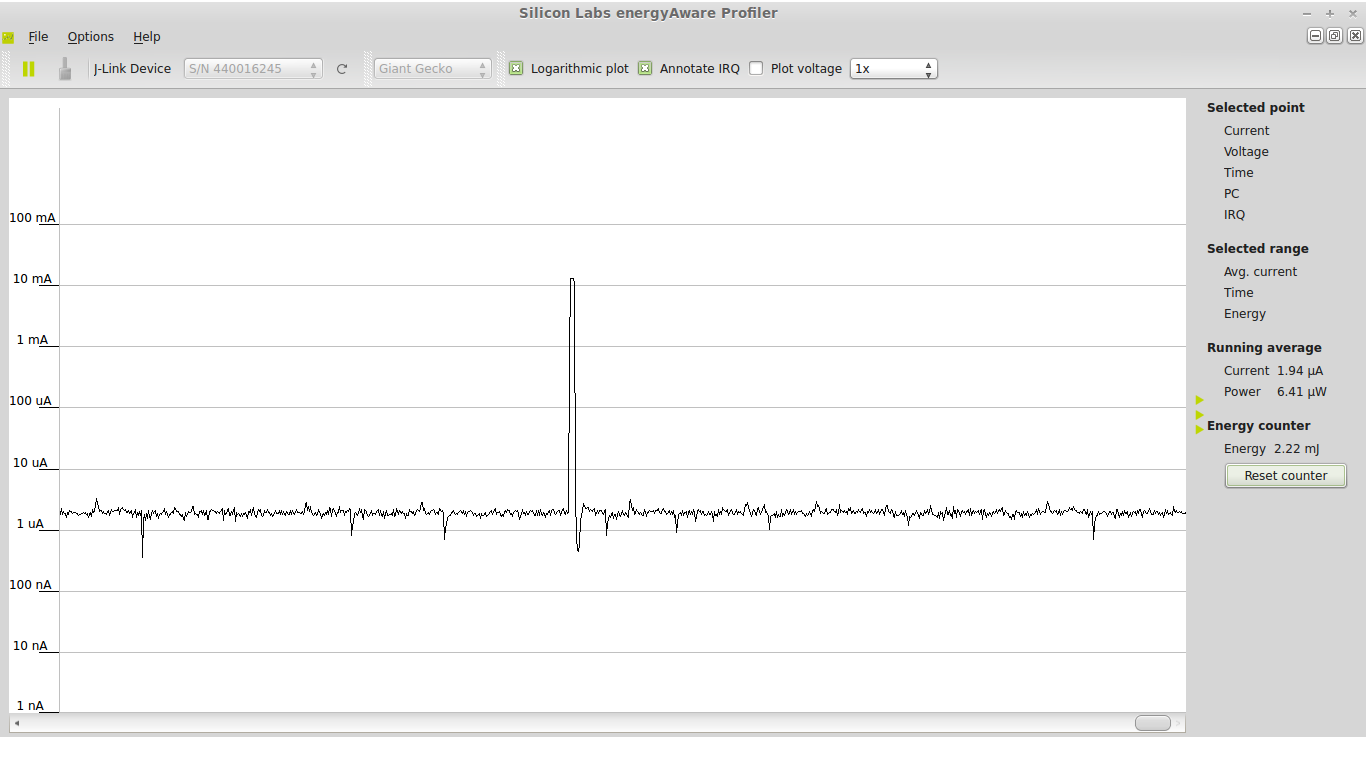
\includegraphics[width=\textwidth]{fig/interruptAndButton.png}	
			\caption{Interrupt with energy mode, button pressed }	
		\end{figure}
	\end{center}	
	
\subsection{Complete system}

The second part of the assignment consisted of implementing a complete system by controlling the LEDs in some way or the other. The two systems created are described in the methodology and the results of the implementation were as follows:

\subsubsection{Blinking LEDs}

\emph{Input: } Specifying the DELAY-variable to 2500 ms. \\
\emph{Expected output: } The four rightmost and four leftmost LEDs take turns on being on, separated by a 2500 ms \\ delay.
\emph{Actual output: } As expected. \\

\subsubsection{Wave}

\emph{Input: } 
\emph{Expected output: }
\emph{Actual output: }



%\subsection{Energy use illustration}
	
%	The following figures illustrates the energy use of the various routines. The last figure shows the spike in energy use when one button is briefly pressed.

%	\begin{center}
%	\begin{figure}[h]
%		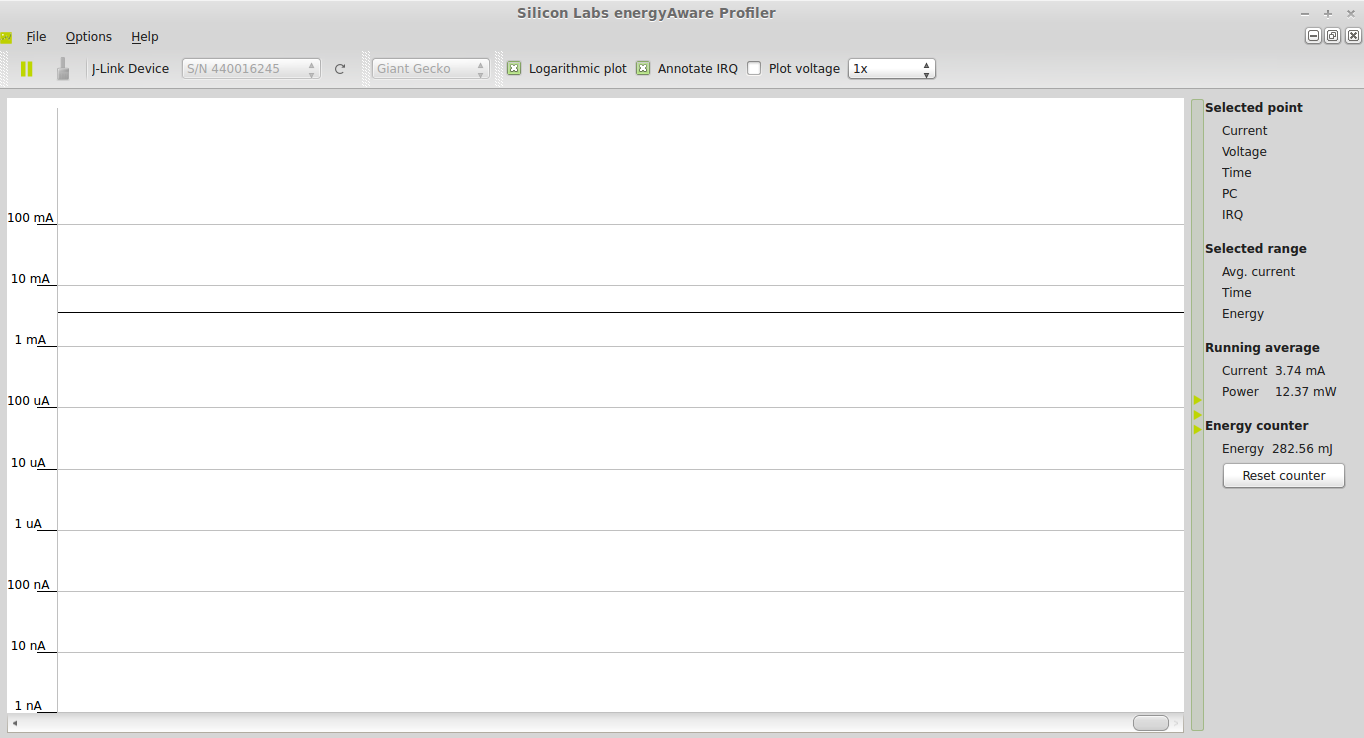
\includegraphics[width=\textwidth]{fig/polling.png}
%		\caption{Polling}
%	\end{figure}

%	\end{center}

	
%	\begin{center}
%		\begin{figure}
		
%		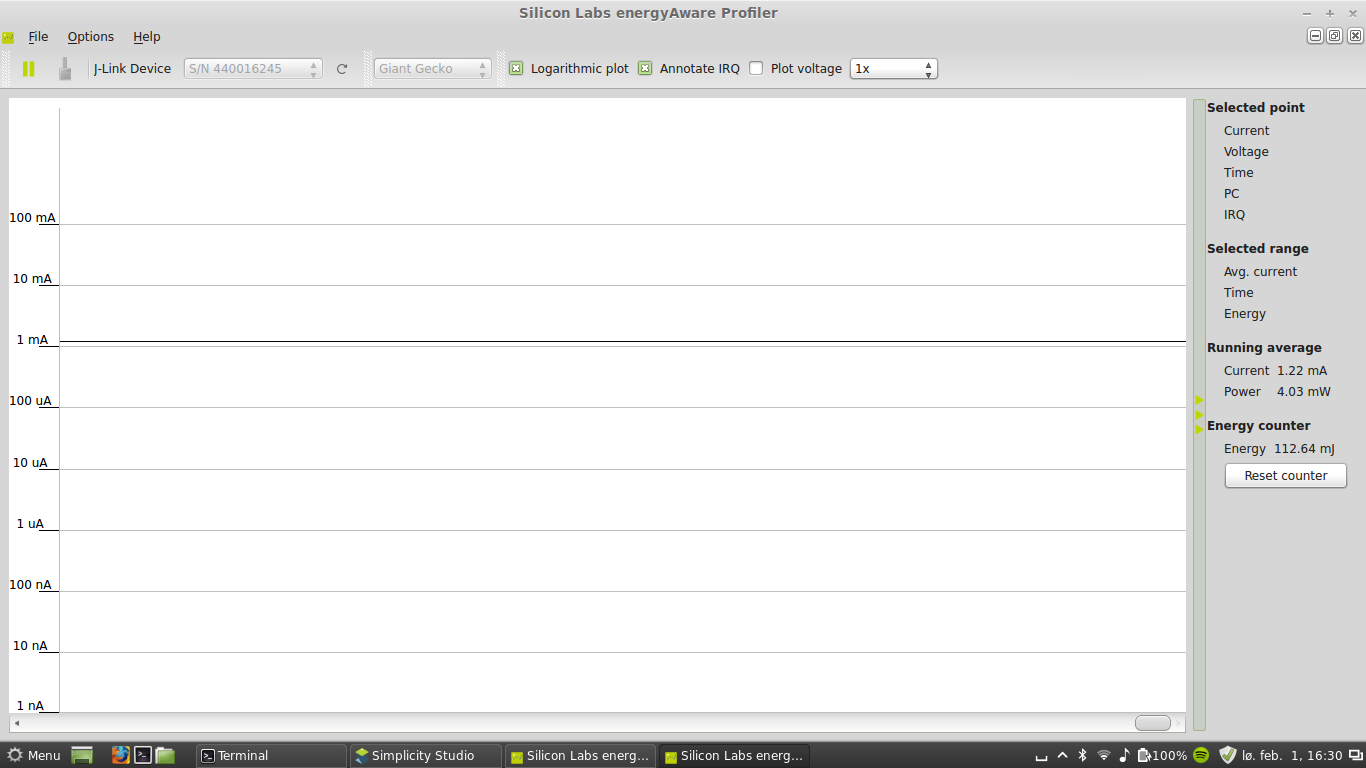
\includegraphics[width=\textwidth]{fig/InterruptOnly.png}
%		\caption{Interrupt without energy mode}
%	\end{figure}
%	\end{center}
%
%	\begin{center}
%	\begin{figure}
	
%	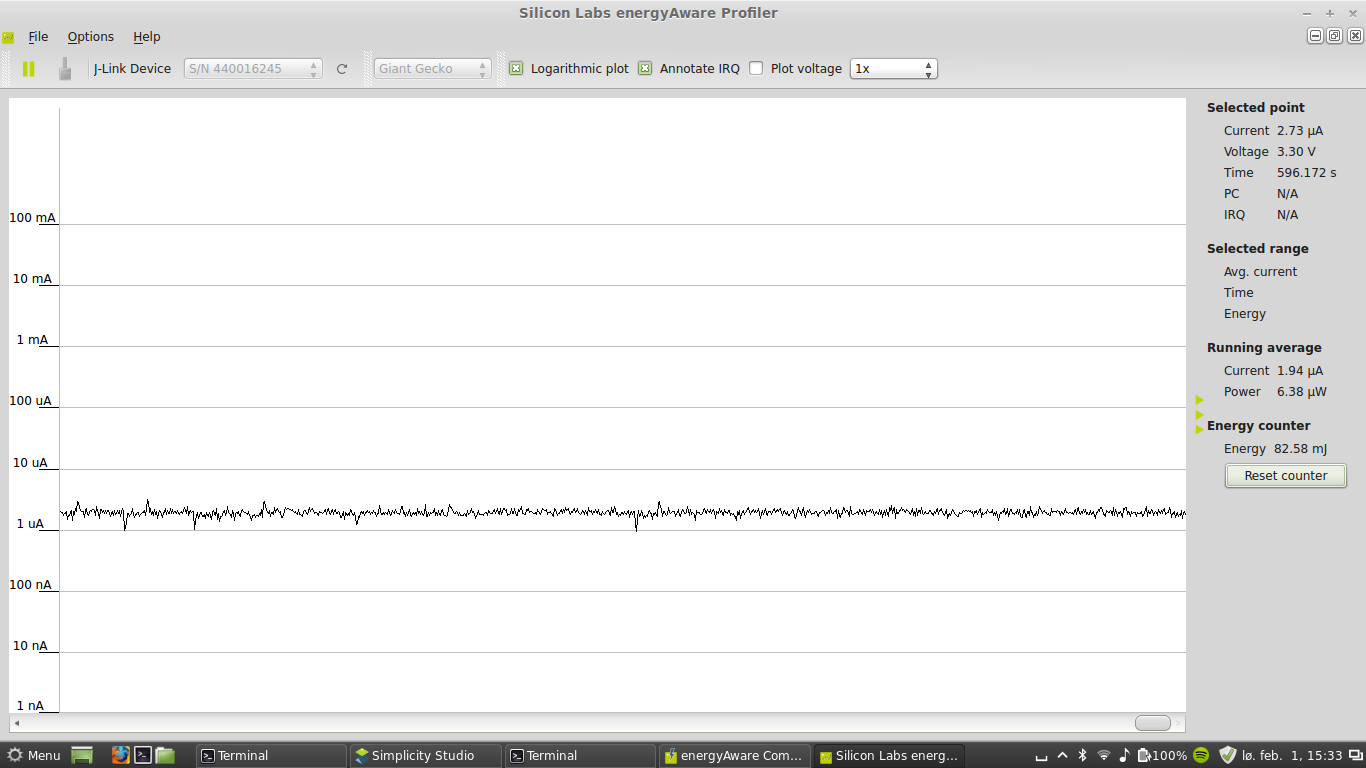
\includegraphics[width=\textwidth]{fig/interruptsAndEnergy.png}	
%	\caption{Interrupt with energy mode}
%	\end{figure}
	
%	\begin{figure}
%	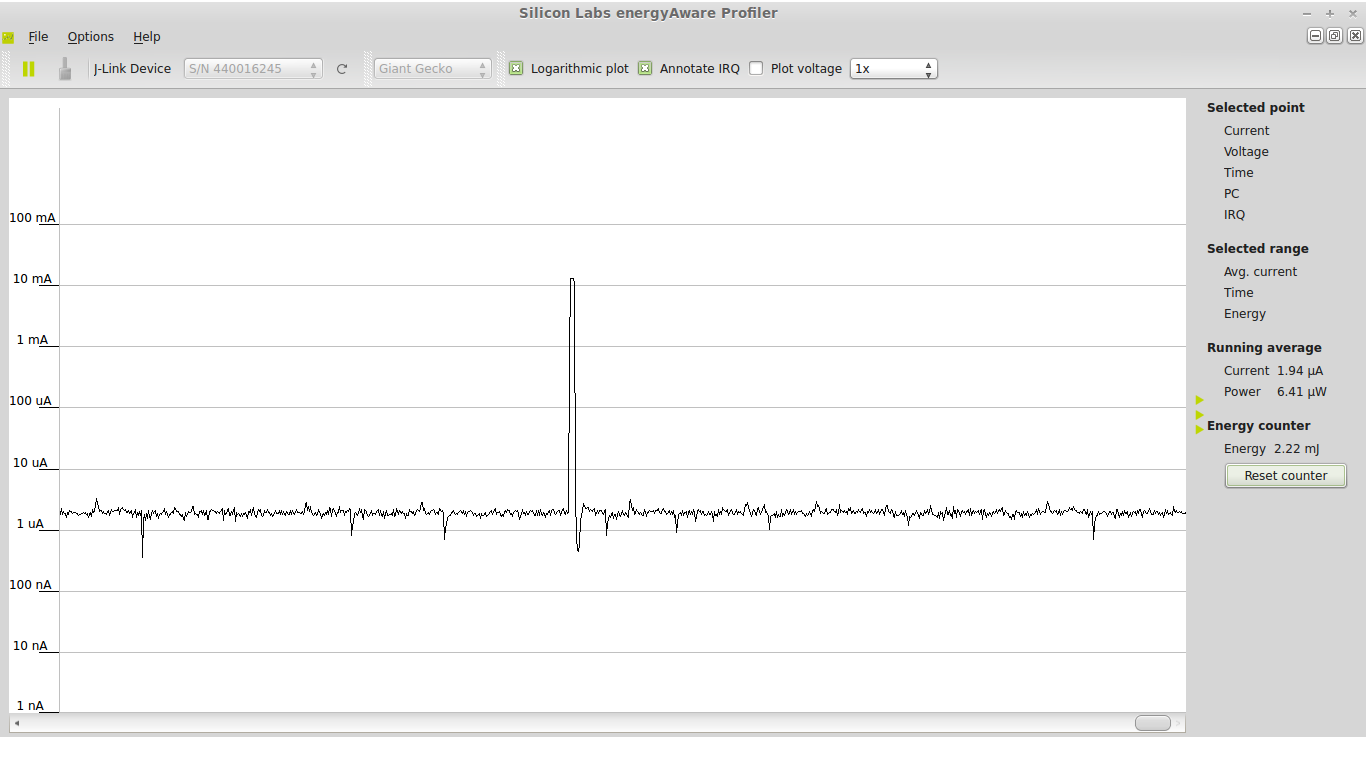
\includegraphics[width=\textwidth]{fig/interruptAndButton.png}	
%	\caption{Interrupt with energy mode, button pressed }	
%	\end{figure}

%	\end{center}